\documentclass{standalone}
\usepackage{graphicx}	
\usepackage{amssymb, amsmath}
\usepackage{color}

\usepackage{tikz}
\usetikzlibrary{intersections, backgrounds, math, decorations.pathreplacing}
\usepackage{pgfmath}

\definecolor{light}{RGB}{220, 188, 188}
\definecolor{mid}{RGB}{185, 124, 124}
\definecolor{dark}{RGB}{143, 39, 39}
\definecolor{highlight}{RGB}{180, 31, 180}
\definecolor{light_teal}{RGB}{107, 142, 142}
\definecolor{mid_teal}{RGB}{72, 117, 117}
\definecolor{dark_teal}{RGB}{29, 79, 79}
\definecolor{gray10}{gray}{0.1}
\definecolor{gray20}{gray}{0.2}
\definecolor{gray30}{gray}{0.3}
\definecolor{gray40}{gray}{0.4}
\definecolor{gray50}{gray}{0.5}
\definecolor{gray60}{gray}{0.6}
\definecolor{gray70}{gray}{0.7}
\definecolor{gray80}{gray}{0.8}
\definecolor{gray90}{gray}{0.9}
\definecolor{gray95}{gray}{0.95}

\tikzmath{
  function f(\x) {
    return sin(100 * \x) + 0.25 * \x;
  };
}

\begin{document}

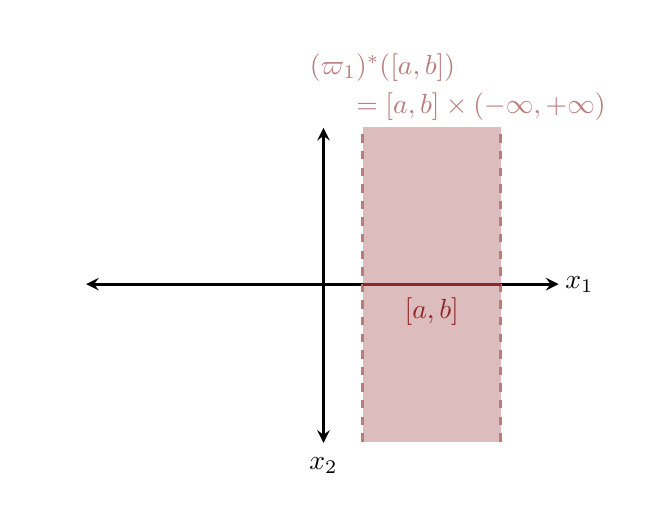
\begin{tikzpicture}[scale=1.0]

  \begin{scope}[shift={(0, 0)}]
    \draw[white] (-3.75, -2.75) rectangle (3.75, 3.25);
   
    \draw [<->, >=stealth, line width=1] (0, -2.015) -- +(0, 4);
    \draw [<->, >=stealth, line width=1] (-3.015, 0.00) -- +(6, 0);
    \node at (0, -2.3) { $x_{2}$ };
    \node at (3.25, 0) { $x_{1}$ };
    
    \fill[light] (0.5, -2) rectangle (2.25, 2);
    \draw[mid, dashed, line width=1] (0.5, -2) -- (0.5, 2);
    \draw[mid, dashed, line width=1] (2.25, -2) -- (2.25, 2);
    \node[mid] at (0.75, 2.75) { $(\varpi_{1})^{*}( [a, b] )$ };
    \node[mid] at (2, 2.25) { $= [a, b] \times (-\infty, +\infty)$ };
    
    \draw[dark, line width=1] (0.5, 0) -- (2.25, 0);
    \node[dark] at (1.375, -0.35) { $[a, b]$ };
                     
  \end{scope}
  
\end{tikzpicture}

\end{document}  